\chapter{Biología del cáncer}\label{ch:b3:cancer-biology}

Un \omterm{def:b3:cancer-biology:hallmarks}{tumor} lo bastante grande como para palparse, de un centímetro, tiene
mil millones de células y es obra de unas treinta duplicaciones a partir
de una célula que se torció --- por lo común una década de crecimiento
antes de que nadie lo supiera. Detrás de esa célula hay varias
mutaciones, cada una de las cuales tuvo que ocurrir en el mismo linaje y
cada una de las cuales eliminó uno de los controles de los dos capítulos
anteriores: un freno de la división, un disparador de la muerte, un
límite al número de divisiones, la obligación de quedarse quieta. El
\omterm{def:b3:cancer-biology:hallmarks}{cáncer} es la evolución de una población celular dentro de un cuerpo, por
mutación y selección, hacia un estado que sirve a las células y mata al
organismo. Este capítulo trata de los genes que resultan tocados y de lo
que hacen normalmente, de la estadística que revela cuántos golpes hacen
falta, de la fisiología que un \omterm{def:b3:cancer-biology:hallmarks}{tumor} ha de adquirir para crecer más allá
de un milímetro y para diseminarse, de las causas que pueden evitarse y
de las terapias --- de los venenos que matan células en división a los
anticuerpos que sueltan al sistema inmunitario --- que la biología ha
hecho posibles, junto con la razón evolutiva por la que fracasan tan a
menudo.

\section{Qué es un cáncer}

\begin{definition}[Tumor, cáncer, rasgos distintivos]\label{def:b3:cancer-biology:hallmarks}
\index{cáncer}\index{tumor}\index{maligno}\index{metástasis}\index{rasgos distintivos del cáncer}
Un \emph{tumor} (neoplasia) es un clon de células que ha escapado a los
controles de su crecimiento y se acumula en un tejido. Es \emph{benigno}
si permanece confinado y encapsulado, y \emph{maligno} --- un
\emph{cáncer} --- si sus células invaden el tejido vecino y siembran
tumores secundarios en otro sitio (la \emph{metástasis}), que es lo que
mata. Los cánceres se nombran por su célula de origen: los carcinomas
proceden de epitelios (el \qty{85}{\%} de los cánceres humanos), los
sarcomas del tejido conjuntivo, las leucemias y los linfomas de las
células formadoras de sangre y los gliomas de la glía. Sea cual sea el
tejido, un clon maligno ha adquirido el mismo conjunto de capacidades,
los \emph{rasgos distintivos del cáncer}: prolifera sin señales externas
de crecimiento e ignora las señales que lo detendrían; resiste a la
\omterm{def:b3:cell-cycle-apoptosis:apoptosis}{apoptosis}; se divide sin límite, tras reactivar la \omterm{def:b3:cancer-biology:telomerase}{telomerasa}; induce
vasos sanguíneos; invade y da metástasis; y, por debajo de todo esto, su
genoma es inestable, reprograma su metabolismo hacia la glicólisis
incluso con oxígeno (el efecto Warburg), recluta células inflamatorias
que lo ayudan y elude al sistema inmunitario. Cada rasgo es un control
del tejido normal derrotado, y cada uno se corresponde con genes.
\end{definition}

\begin{omfigure}
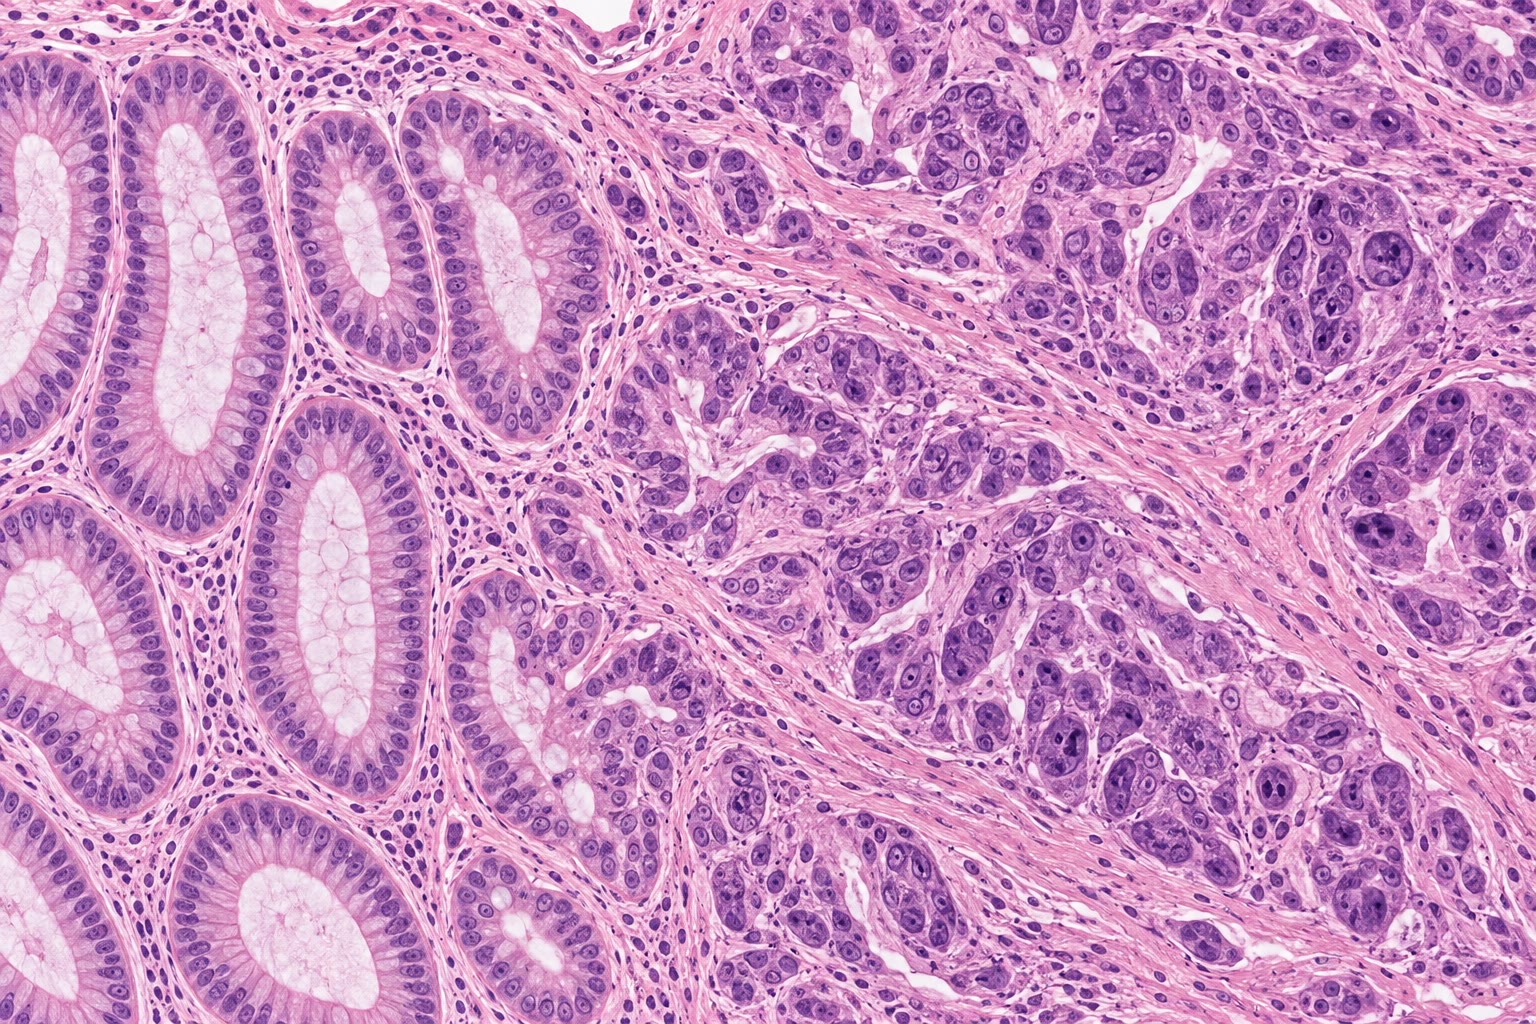
\includegraphics[width=0.56\linewidth]{images/book5/ai/b5-11-tumour-histology.jpg}

{\small Un carcinoma en su borde: a la izquierda, un epitelio glandular
ordenado con núcleos regulares; a la derecha, células apiñadas con
núcleos grandes e irregulares que invaden el estroma subyacente --- la
imagen que lee un patólogo para llamar \omterm{def:b3:cancer-biology:hallmarks}{maligno} a un \omterm{def:b3:cancer-biology:hallmarks}{tumor}.}
\end{omfigure}

\section{Los genes que resultan tocados}

\begin{definition}[Oncogenes y supresores de tumores]\label{def:b3:cancer-biology:genes}
\index{oncogén}\index{protooncogén}\index{gen supresor de tumores}\index{Ras}\index{p53}\index{hipótesis de los dos golpes}
Un \emph{protooncogén} es un gen normal que favorece la proliferación o
la supervivencia --- un factor de crecimiento, su receptor, una proteína
de señalización, un factor de transcripción, una \omterm{def:b3:cell-cycle-apoptosis:cdk}{ciclina} ---, y un
\emph{oncogén} es una forma mutante que está activa sin su señal normal:
una mutación puntual que bloquea a la \omterm{def:b3:membrane-traffic:coats}{GTPasa pequeña} \emph{Ras} en su
estado con GTP (la glicina~12 en una cuarta parte de todos los \omterm{def:b3:cancer-biology:hallmarks}{cánceres}),
una amplificación del gen del receptor HER2 o del factor de
transcripción Myc, una translocación que fusiona \emph{BCR} con la
quinasa \emph{ABL} en la leucemia mieloide crónica o que coloca a
\emph{MYC} junto a un potenciador de anticuerpos en el linfoma de
Burkitt. Basta con un alelo mutante: los oncogenes actúan de forma
dominante. Un \emph{gen supresor de \omterm{def:b3:cancer-biology:hallmarks}{tumores}} frena la proliferación o
impone la muerte o la reparación --- Rb y p16 en el \omterm{def:b3:cell-cycle-apoptosis:checkpoints}{punto de
restricción}, \emph{p53}, el guardián que detiene o mata a una célula
dañada, APC en la \omterm{prop:b3:cancer-biology:pathways}{vía Wnt} del colon, PTEN, BRCA1 y BRCA2, los genes de la
\omterm{prop:b3:dna-repair:fidelity}{reparación de errores de apareamiento} --- y ha de perder los dos alelos
para contribuir: \emph{dos golpes}, el primero de ellos heredado a menudo
en los síndromes de \omterm{def:b3:cancer-biology:hallmarks}{cáncer} familiar y el segundo somático. \emph{p53}
está mutado en la mitad de todos los \omterm{def:b3:cancer-biology:hallmarks}{cánceres} humanos y su vía
inutilizada en casi todos los demás.
\end{definition}

\begin{proof}[Evidencia]
Rous (1911) transmitió un sarcoma de gallina con un filtrado libre de
células, un virus, cuyo único gen transformante, \emph{src}, mostraron
Varmus y Bishop (1976) que era una copia capturada de un gen normal de
gallina --- los oncogenes son genes celulares alterados. Weinberg (1982)
transfirió ADN de un carcinoma humano de vejiga a células de ratón en
cultivo, que quedaron transformadas; el fragmento responsable era
\emph{RAS} con un solo cambio de base, y ese mismo cambio estaba ausente
del tejido normal del paciente. Knudson (1971) comparó niños con el \omterm{def:b3:cancer-biology:hallmarks}{tumor}
ocular retinoblastoma: los que tenían antecedentes familiares
desarrollaban varios \omterm{def:b3:cancer-biology:hallmarks}{tumores} en ambos ojos, y pronto; los que no,
desarrollaban uno, y más tarde --- coherente con que los casos familiares
necesiten un suceso somático y los esporádicos dos, y por tanto con un
gen cuyas dos copias han de perderse ambas. \emph{RB} se clonó en 1986 y
en todos los \omterm{def:b3:cancer-biology:hallmarks}{tumores} estaban en efecto inactivados los dos alelos.
\end{proof}

\begin{theorem}[Golpes y la curva de edad]\label{thm:b3:cancer-biology:armitage-doll}
\index{modelo de Armitage--Doll}\index{carcinogénesis multietapa}
Supóngase que un \omterm{def:b3:cancer-biology:hallmarks}{cáncer} exige $k$ sucesos independientes y limitantes en
un mismo linaje celular, cada uno con una velocidad constante $u$ por
célula y año, en una población de $N$ células susceptibles, con
$ut \ll 1$. Entonces la probabilidad de que una célula dada haya sufrido
los $k$ sucesos a la edad $t$ es aproximadamente $(ut)^{k}$, el riesgo
acumulado del tejido es aproximadamente $N(ut)^{k}$, y la incidencia ---
casos nuevos por año a la edad $t$ --- es
\[
I(t) \approx N\,k\,u^{k}\,t^{\,k-1},
\]
una potencia de la edad de exponente $k - 1$: una recta de pendiente
$k - 1$ en un gráfico logarítmico doble. Para quien hereda uno de los
sucesos, el mismo \omterm{def:b3:cancer-biology:hallmarks}{cáncer} tiene una incidencia $\propto t^{\,k-2}$, una
potencia menos.
\end{theorem}
\begin{proof}
Cada suceso, a velocidad $u$, ha ocurrido en el instante $t$ con
probabilidad $1 - e^{-ut} \approx ut$; los sucesos son independientes, de
modo que los $k$ han ocurrido con probabilidad $(ut)^{k}$, y el orden en
que ocurrieron no importa aquí. Con $N$ células y sucesos raros, el
número esperado de células que han completado la secuencia es
$N(ut)^{k}$, y la incidencia es su derivada temporal, $Nku^{k}t^{k-1}$.
Heredar un suceso deja $k - 1$ por ocurrir: $(ut)^{k-1}$, con incidencia
$\propto t^{k-2}$. Si el orden de los sucesos importara (solo $1$ de los
$k!$ órdenes lleva al \omterm{def:b3:cancer-biology:hallmarks}{cáncer}), cambiaría el prefactor, no el exponente.
\end{proof}

\begin{example}[Leer el exponente]\label{ex:b3:cancer-biology:exponent}
La incidencia de la mayoría de los carcinomas en el adulto sube como la
quinta o sexta potencia de la edad --- de aproximadamente $1$ de cada
\num{100000} al año a los treinta a $1$ de cada $300$ a los ochenta, un
factor de $300$ para un factor $2.7$ en la edad, y
$2.7^{5.7} \approx 300$ ---, lo que sugiere seis o siete sucesos
limitantes. La estimación es tosca: la expansión de un clon tras cada
golpe eleva el número de células en riesgo del siguiente, de modo que
menos sucesos con crecimiento clonal entre ellos dan la misma pendiente,
y el número de mutaciones \emph{conductoras} que se encuentran en los
\omterm{def:b3:cancer-biology:hallmarks}{tumores} secuenciados es de dos a ocho. El retinoblastoma de Knudson
encaja exactamente en la segunda afirmación del teorema: la enfermedad
esporádica, que necesita dos golpes, tiene una incidencia que sube con la
edad (a lo largo de los pocos años en que existen los retinoblastos); la
hereditaria, que necesita uno, está presente a una tasa casi constante
desde el nacimiento y golpea pronto y repetidamente.
\end{example}

\begin{omfigure}
\begin{tikzpicture}
\begin{axis}[
  width=0.68\linewidth, height=6cm,
  xmode=log, ymode=log,
  xmin=20, xmax=100, ymin=1e-6, ymax=1e-1,
  xlabel={edad (años)}, ylabel={incidencia por persona y año},
  xlabel style={font=\small, at={(axis description cs:0.5,-0.12)}, anchor=north},
  ylabel style={font=\small},
  tick label style={font=\small}, xtick={20,30,50,80}, xticklabels={20,30,50,80},
  clip=false,
]
\addplot[very thick, omThm, domain=20:100, samples=2] {1e-5*(x/30)^5.7};
\addplot[very thick, omDef, domain=20:100, samples=2] {3e-4*(x/30)^1};
\addplot[very thick, omMeth!70!black, domain=20:100, samples=2] {2e-3};
\node[font=\scriptsize, omThm, anchor=south west] at (axis cs:38,2.5e-6) {carcinomas: pendiente $5$--$6$, seis o siete sucesos};
\node[font=\scriptsize, omDef, anchor=south west] at (axis cs:22,6e-4) {dos golpes: pendiente 1};
\node[font=\scriptsize, omMeth!70!black, anchor=south west] at (axis cs:22,2.3e-3) {un golpe heredado: pendiente 0};
\end{axis}
\end{tikzpicture}

{\small Incidencia frente a edad en ejes logarítmicos. Un \omterm{def:b3:cancer-biology:hallmarks}{cáncer} que
necesita $k$ sucesos limitantes sube como $t^{k-1}$: la recta empinada de
los carcinomas del adulto y los dos casos de Knudson --- un \omterm{def:b3:cancer-biology:hallmarks}{tumor} de dos
golpes que sube linealmente, y ese mismo \omterm{def:b3:cancer-biology:hallmarks}{tumor} en un portador de un golpe
heredado, a tasa constante desde el nacimiento.}
\end{omfigure}

\begin{proposition}[Las vías que resultan tocadas]\label{prop:b3:cancer-biology:pathways}
\index{vía Ras--MAPK}\index{vía PI3K}\index{vía Wnt}
Los centenares de genes del \omterm{def:b3:cancer-biology:hallmarks}{cáncer} se reparten en una docena de vías, y
cada \omterm{def:b3:cancer-biology:hallmarks}{tumor} inutiliza una de ellas en algún punto. Las vías de los
factores de crecimiento: un receptor con actividad tirosina-quinasa
(EGFR, HER2), \omterm{def:b3:cancer-biology:genes}{Ras}, la cascada de quinasas Raf--MEK--ERK hacia el núcleo
y, en paralelo, PI3K--Akt--mTOR hacia la supervivencia y el crecimiento,
frenada por PTEN; un \omterm{def:b3:cancer-biology:hallmarks}{tumor} activa una de ellas, por el gen que sea. El
freno del \omterm{def:b3:cell-cycle-apoptosis:cdk}{ciclo celular}: la \omterm{def:b3:cell-cycle-apoptosis:cdk}{ciclina} D, Cdk4, p16 y Rb
(\cref{ch:b3:cell-cycle-apoptosis}). El guardián: \omterm{def:b3:cancer-biology:genes}{p53} y sus reguladores.
La muerte: Bcl-2. La señalización del desarrollo: Wnt (APC,
$\beta$-catenina) en el colon, Hedgehog en la piel y el cerebro, Notch en
los linfocitos~T. El mantenimiento del genoma: la \omterm{prop:b3:dna-repair:fidelity}{reparación de errores
de apareamiento}, \omterm{def:b3:dna-repair:dsb}{BRCA}, \omterm{def:b3:dna-repair:ddr}{ATM}. La \omterm{def:b3:chromatin-epigenetics:nucleosome}{cromatina}: los escritores y
remodeladores del \cref{ch:b3:chromatin-epigenetics}, mutados en un
tercio de los \omterm{def:b3:cancer-biology:hallmarks}{tumores}. La inmortalidad: el promotor de la \omterm{def:b3:cancer-biology:telomerase}{telomerasa}.
Como una vía es una serie de pasos, las mutaciones de genes distintos son
alternativas --- un \omterm{def:b3:cancer-biology:hallmarks}{tumor} con \omterm{def:b3:cancer-biology:genes}{Ras} mutante rara vez tiene además un EGFR
mutante --- y los fármacos contra un paso pueden ser derrotados por una
mutación aguas abajo.
\end{proposition}

\begin{omfigure}
\begin{tikzpicture}[every node/.style={font=\scriptsize}, >=stealth]
  % membrane
  \draw[very thick, omDef] (0,3.6) -- (12,3.6); \draw[very thick, omDef] (0,3.3) -- (12,3.3);
  \node[above] at (1.0,3.65) {exterior}; \node[below] at (1.0,3.25) {citosol};
  % receptor
  \draw[thick, fill=omProp!35] (3.7,3.0) rectangle (4.1,4.1); \draw[thick, fill=omProp!35] (4.3,3.0) rectangle (4.7,4.1);
  \node[above, align=center] at (4.2,4.15) {factor de crecimiento $\to$ receptor quinasa\\(EGFR, HER2)}; \node[right, omThm, font=\tiny] at (4.75,4.0) {amplificado};
  % Ras
  \node[draw, thick, rounded corners, fill=omDef!20] (ras) at (4.2,2.3) {Ras--GTP};
  \node[right, omThm, font=\tiny] at (5.0,2.3) {G12: siempre activa};
  \node[draw, thick, rounded corners, fill=omDef!20] (raf) at (4.2,1.4) {Raf $\to$ MEK $\to$ ERK};
  \node[right, omThm, font=\tiny] at (5.8,1.4) {BRAF V600E};
  \node[draw, thick, rounded corners, fill=omMeth!25] (myc) at (4.2,0.4) {Myc, ciclina D: proliferación};
  \node[right, omThm, font=\tiny] at (6.4,0.4) {Myc amplificado};
  \draw[->, thick] (4.2,3.0) -- (ras); \draw[->, thick] (ras) -- (raf); \draw[->, thick] (raf) -- (myc);
  % PI3K branch
  \node[draw, thick, rounded corners, fill=omDef!20] (pi3k) at (9.6,2.3) {PI3K $\to$ Akt $\to$ mTOR};
  \node[draw, thick, rounded corners, fill=omMeth!25] (surv) at (9.6,0.4) {supervivencia, crecimiento};
  \draw[->, thick] (4.7,3.0) .. controls (6.5,2.8) .. (pi3k.north west); \draw[->, thick] (pi3k) -- (surv);
  \node[draw, thick, rounded corners, fill=omThm!15] (pten) at (12.2,1.4) {PTEN}; \draw[-|, thick, omThm] (pten) -- (9.6,1.4);
  \node[below, omThm, font=\tiny] at (12.2,1.15) {delecionado};
  % p53 and Rb on the side
  \node[draw, thick, rounded corners, fill=omThm!15] (rb) at (1.2,0.4) {Rb, p16}; \draw[-|, thick, omThm] (rb) -- (myc);
  \node[below, omThm, font=\tiny, align=center] at (1.2,0.15) {ambos alelos perdidos};
  \node[draw, thick, rounded corners, fill=omThm!15] (p53) at (1.2,1.6) {p53}; \node[below, omThm, font=\tiny, align=center] at (1.2,1.35) {mutado en la mitad\\de los cánceres};
  \draw[-|, thick, omThm] (p53) -- (1.2,0.65);
\end{tikzpicture}

{\small Las vías de los factores de crecimiento y dónde las golpean los
\omterm{def:b3:cancer-biology:hallmarks}{cánceres}. Las cajas verdes son las salidas, las azules los pasos de
señalización que las mutaciones oncogénicas dejan encendidos y las rojas
los supresores que los \omterm{def:b3:cancer-biology:hallmarks}{tumores} pierden (las barras marcan inhibición). Un
\omterm{def:b3:cancer-biology:hallmarks}{tumor} lleva típicamente una lesión activadora y una o dos inactivadoras
de este diagrama.}
\end{omfigure}

\section{Un tumor evoluciona}

\begin{proposition}[Carcinogénesis en varias etapas]\label{prop:b3:cancer-biology:multistep}
\index{mutación conductora}\index{mutación pasajera}\index{evolución clonal}\index{firma mutacional}
Un \omterm{def:b3:cancer-biology:hallmarks}{tumor} es el producto de una evolución somática: la mutación genera
variantes y la selección dentro del tejido favorece a las que se dividen
más, mueren menos o escapan a una restricción. La secuencia colorrectal
que estableció Vogelstein es el paradigma: la pérdida de \emph{APC}
produce un pólipo benigno pequeño; una mutación de \emph{KRAS} le permite
crecer hasta un adenoma; la pérdida de \emph{SMAD4} o de \emph{TP53} lo
convierte en un carcinoma; y cambios posteriores permiten la \omterm{def:b3:cancer-biology:metastasis}{invasión}.
Cada paso es una expansión clonal que multiplica las células en riesgo
del siguiente. Un \omterm{def:b3:cancer-biology:hallmarks}{tumor} secuenciado lleva miles de mutaciones, de las que
un puñado --- típicamente de dos a ocho --- son \emph{conductoras} que
confirieron ventaja selectiva; el resto son \emph{pasajeras},
arrastradas por el clon, y su espectro es un registro de lo que las
causó: C$\to$T en pirimidinas contiguas por la luz ultravioleta en el
melanoma, G$\to$T por el humo del tabaco en el \omterm{def:b3:cancer-biology:hallmarks}{cáncer} de pulmón, las
huellas de las enzimas APOBEC, de una \omterm{prop:b3:dna-repair:fidelity}{reparación de errores de
apareamiento} defectuosa, de la aflatoxina --- las \emph{\omterm{prop:b3:cancer-biology:multistep}{firmas
mutacionales}}. Los \omterm{def:b3:cancer-biology:hallmarks}{tumores} son heterogéneos, un árbol ramificado de
subclones, y el subclon que mata es a menudo minoritario en el
diagnóstico.
\end{proposition}

\begin{omfigure}
\begin{tikzpicture}[every node/.style={font=\scriptsize}, >=stealth]
  \foreach \x/\lab/\gene/\col/\r in {0/{epitelio normal}/{}/omDef!20/0.5, 2.6/{pólipo pequeño}/{APC perdido (ambos alelos)}/omDef!35/0.7, 5.4/adenoma/{KRAS activado}/omProp!40/1.0, 8.4/carcinoma/{SMAD4 o TP53 perdidos}/omThm!35/1.3, 11.6/{invasivo, metastásico}/{más conductoras,\\inestabilidad}/omThm!60/1.5} {
    \draw[thick, fill=\col] (\x,0) circle (\r);
    \node[below, align=center] at (\x,-1.6) {\lab};
    \node[above, align=center, omThm] at (\x,1.6) {\gene};
  }
  \foreach \a/\b in {0.5/1.9, 3.3/4.4, 6.4/7.1, 9.7/10.1} \draw[->, very thick] (\a,0) -- (\b,0);
  \node[below] at (5.8,-2.3) {de diez a treinta años; cada paso una expansión clonal que multiplica las células en riesgo del siguiente};
\end{tikzpicture}

{\small La secuencia colorrectal. Cada \omterm{prop:b3:cancer-biology:multistep}{mutación conductora} expande un
clon, y el clon expandido aporta las células en las que puede surgir la
conductora siguiente; todo el camino tarda décadas, que es por lo que
cribar pólipos previene el \omterm{def:b3:cancer-biology:hallmarks}{cáncer}.}
\end{omfigure}

\begin{method}[La prueba de Ames]\label{met:b3:cancer-biology:ames}
\index{prueba de Ames}\index{mutágeno}
Para comprobar si una sustancia química es mutagénica y, por tanto,
probablemente carcinógena: (1) tómese una cepa de \emph{Salmonella} con
una mutación puntual en un gen de la biosíntesis de histidina, que no
puede crecer sin histidina; (2) mézclese la sustancia con un extracto de
hígado, cuyas enzimas convierten muchos compuestos en sus formas
mutagénicas activas, como haría el cuerpo; (3) siémbrense unas $10^{8}$
bacterias en agar sin histidina con la mezcla; (4) cuéntense las colonias
que crezcan --- cada una es una revertiente en la que una mutación nueva
ha restaurado el gen; (5) compárese con la tasa espontánea. Un aumento de
revertientes dependiente de la dosis significa que el compuesto causa
mutaciones puntuales. Casi todos los carcinógenos conocidos dan positivo;
la prueba es barata, dura dos días, y un compuesto que no la pasa se
examina más a fondo antes de fabricarse.
\end{method}

\begin{definition}[Inmortalidad e inestabilidad]\label{def:b3:cancer-biology:telomerase}
\index{telomerasa}\index{inestabilidad cromosómica}\index{aneuploidía!en el cáncer}
Las células somáticas normales carecen de telomerasa y cuentan sus
divisiones en la longitud de los telómeros (\cref{ch:b3:stem-cells}):
tras unas cincuenta entran en \omterm{def:b3:cell-cycle-apoptosis:other}{senescencia}, y una célula que sortea la
\omterm{def:b3:cell-cycle-apoptosis:other}{senescencia} perdiendo \omterm{def:b3:cancer-biology:genes}{p53} y Rb sigue adelante hasta que sus telómeros se
agotan y sus cromosomas se fusionan y se rompen --- una crisis que mata a
casi todos los clones. El raro superviviente ha reactivado la
\emph{telomerasa}, por lo general mediante una mutación del promotor, y
es inmortal; el \qty{90}{\%} de los \omterm{def:b3:cancer-biology:hallmarks}{cánceres} expresan la enzima. La
crisis deja cicatrices: cromosomas fusionados y rotos, amplificaciones,
deleciones, translocaciones --- la \emph{inestabilidad cromosómica} que,
junto con la pérdida del punto de control del huso y de la respuesta de
\omterm{def:b3:cancer-biology:genes}{p53} a la mala segregación, hace aneuploides a la mayoría de los \omterm{def:b3:cancer-biology:hallmarks}{tumores}
sólidos y los mantiene generando variantes. Una minoría de \omterm{def:b3:cancer-biology:hallmarks}{tumores} tiene
en cambio un fenotipo mutador por pérdida de la \omterm{prop:b3:dna-repair:fidelity}{reparación de errores de
apareamiento}, con un cariotipo normal y una tasa de mutación puntual mil
veces mayor.
\end{definition}

\section{El tumor como tejido}

\begin{proposition}[El oxígeno fija el tamaño de un tumor sin vasos]\label{prop:b3:cancer-biology:oxygen}
\index{angiogénesis}\index{límite de difusión}\index{hipoxia}
Considérese un tejido que consume oxígeno a velocidad constante $q$ por
unidad de volumen, abastecido por difusión (coeficiente $D$) desde un
vaso en cuya pared la concentración es $c_{0}$. En una dimensión y en el
estado estacionario, $D\,
\mathrm{d}^{2}c/\mathrm{d}x^{2} = q$, de modo que
$c(x) = c_{0} - qx^{2}/2D$ y el oxígeno se agota a la distancia
\[
L = \sqrt{\frac{2Dc_{0}}{q}} .
\]
Con $D = \qty{2e-9}{m^2/s}$, $c_{0} = \qty{0.05}{mol/m^3}$ y $q =
\qty{0.03}{mol/m^3/s}$ (un \omterm{def:b3:cancer-biology:hallmarks}{tumor} que respira), $L \approx \qty{80}{\micro
m}$: ninguna célula puede vivir a más de unos cien micrómetros de un
capilar. Un clon sin vasos propios se detiene por tanto en un diámetro de
uno o dos milímetros, con el centro necrótico y el borde vivo. Para
crecer más ha de inducir la \emph{angiogénesis} --- sus células
hipóxicas estabilizan el factor de transcripción HIF, que induce el VEGF,
que hace brotar hacia él a las células endoteliales cercanas. Judah
Folkman propuso en 1971 que bloquear ese paso mataría de hambre a los
\omterm{def:b3:cancer-biology:hallmarks}{tumores}; los anticuerpos contra el VEGF son hoy habituales en varios
\omterm{def:b3:cancer-biology:hallmarks}{cánceres}, aunque los \omterm{def:b3:cancer-biology:hallmarks}{tumores} se adaptan.
\end{proposition}
\begin{proof}
En el estado estacionario el flujo difusivo $-D\,\mathrm{d}c/\mathrm{d}x$
ha de cambiar con $x$ exactamente tan deprisa como se consume el oxígeno:
$\mathrm{d}(-D\,
\mathrm{d}c/\mathrm{d}x)/\mathrm{d}x = -q$, es decir, $D c'' = q$.
Integrando dos veces con $c(0) = c_{0}$ y $c'(L) = 0$ a la profundidad
donde no queda nada (sin flujo más allá) se obtiene
$c = c_{0} - qx^{2}/2D$, tras usar $c(L) = 0$ para fijar $L$. Los números
se siguen.
\end{proof}

\begin{omfigure}
\begin{tikzpicture}
\begin{axis}[
  width=0.6\linewidth, height=5.4cm,
  axis x line=bottom, axis y line=left,
  xmin=0, xmax=120, ymin=0, ymax=0.06,
  xlabel={distancia al capilar ($\unit{\micro m}$)}, ylabel={oxígeno ($\unit{mol/m^3}$)},
  xlabel style={font=\small, at={(axis description cs:0.5,-0.12)}, anchor=north},
  ylabel style={font=\small},
  tick label style={font=\small}, xtick={0,40,80,120}, ytick={0,0.025,0.05},
  clip=false,
]
\addplot[very thick, omDef, domain=0:81.6, samples=40] {0.05 - 0.03*(x*1e-6)^2/(2*2e-9)};
\addplot[very thick, omDef, domain=81.6:120, samples=2] {0};
\fill[omThm!25] (axis cs:81.6,0) rectangle (axis cs:120,0.06);
\node[font=\scriptsize, omThm!70!black, anchor=south, align=center] at (axis cs:100,0.03) {sin oxígeno:\\necrosis};
\node[font=\scriptsize, omDef, anchor=south west] at (axis cs:5,0.052) {$c(x) = c_{0} - qx^{2}/2D$};
\draw[dashed, gray] (axis cs:81.6,0) -- (axis cs:81.6,0.06); \node[font=\scriptsize, anchor=south west] at (axis cs:83,0.002) {$L$};
\end{axis}
\end{tikzpicture}

{\small El oxígeno de un tejido que respira cae como una parábola con la
distancia al capilar más próximo y se agota en $L = \sqrt{2Dc_{0}/q}$,
aquí unos \qty{80}{\micro m}. Un \omterm{def:b3:cancer-biology:hallmarks}{tumor} sin vasos es una corteza de
células vivas de ese espesor en torno a un núcleo muerto.}
\end{omfigure}

\begin{omfigure}
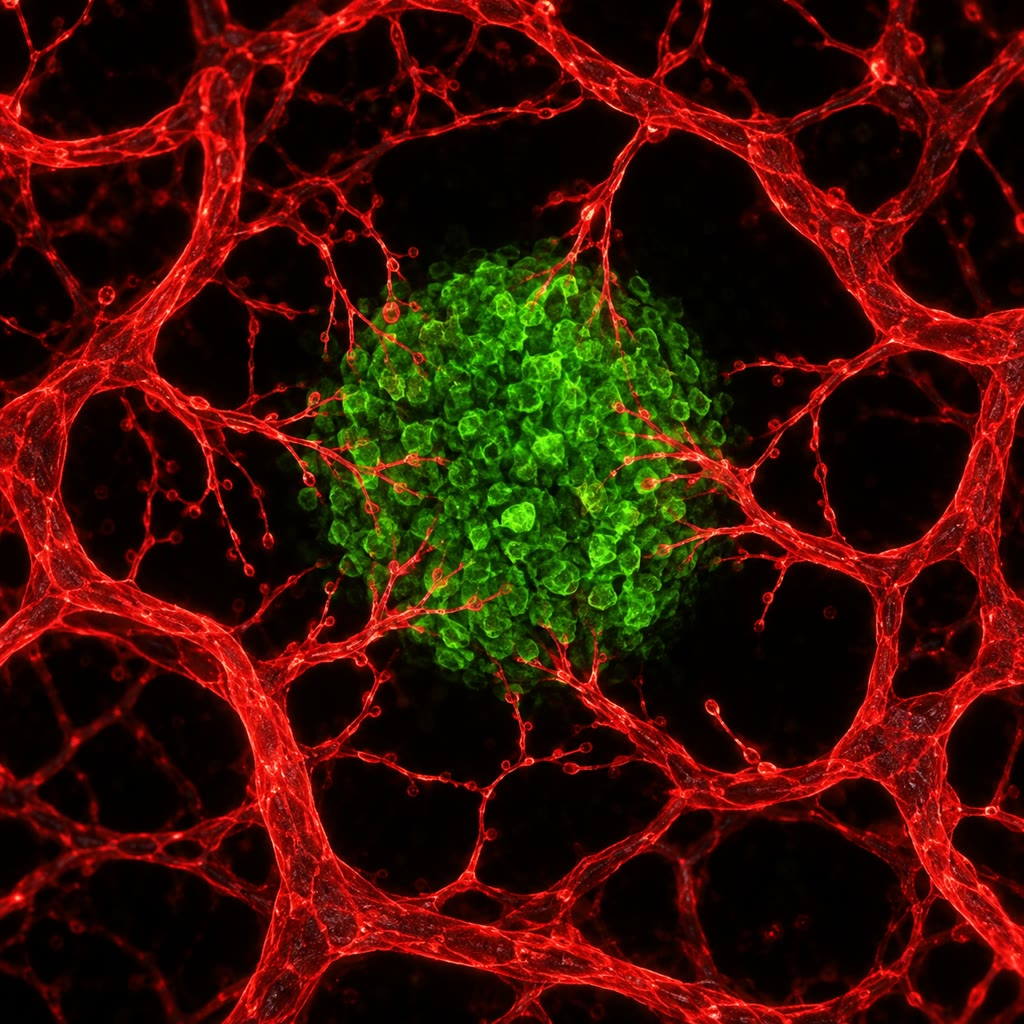
\includegraphics[width=0.36\linewidth]{images/book5/ai/b5-11-angiogenesis.jpg}\hspace{0.04\linewidth}
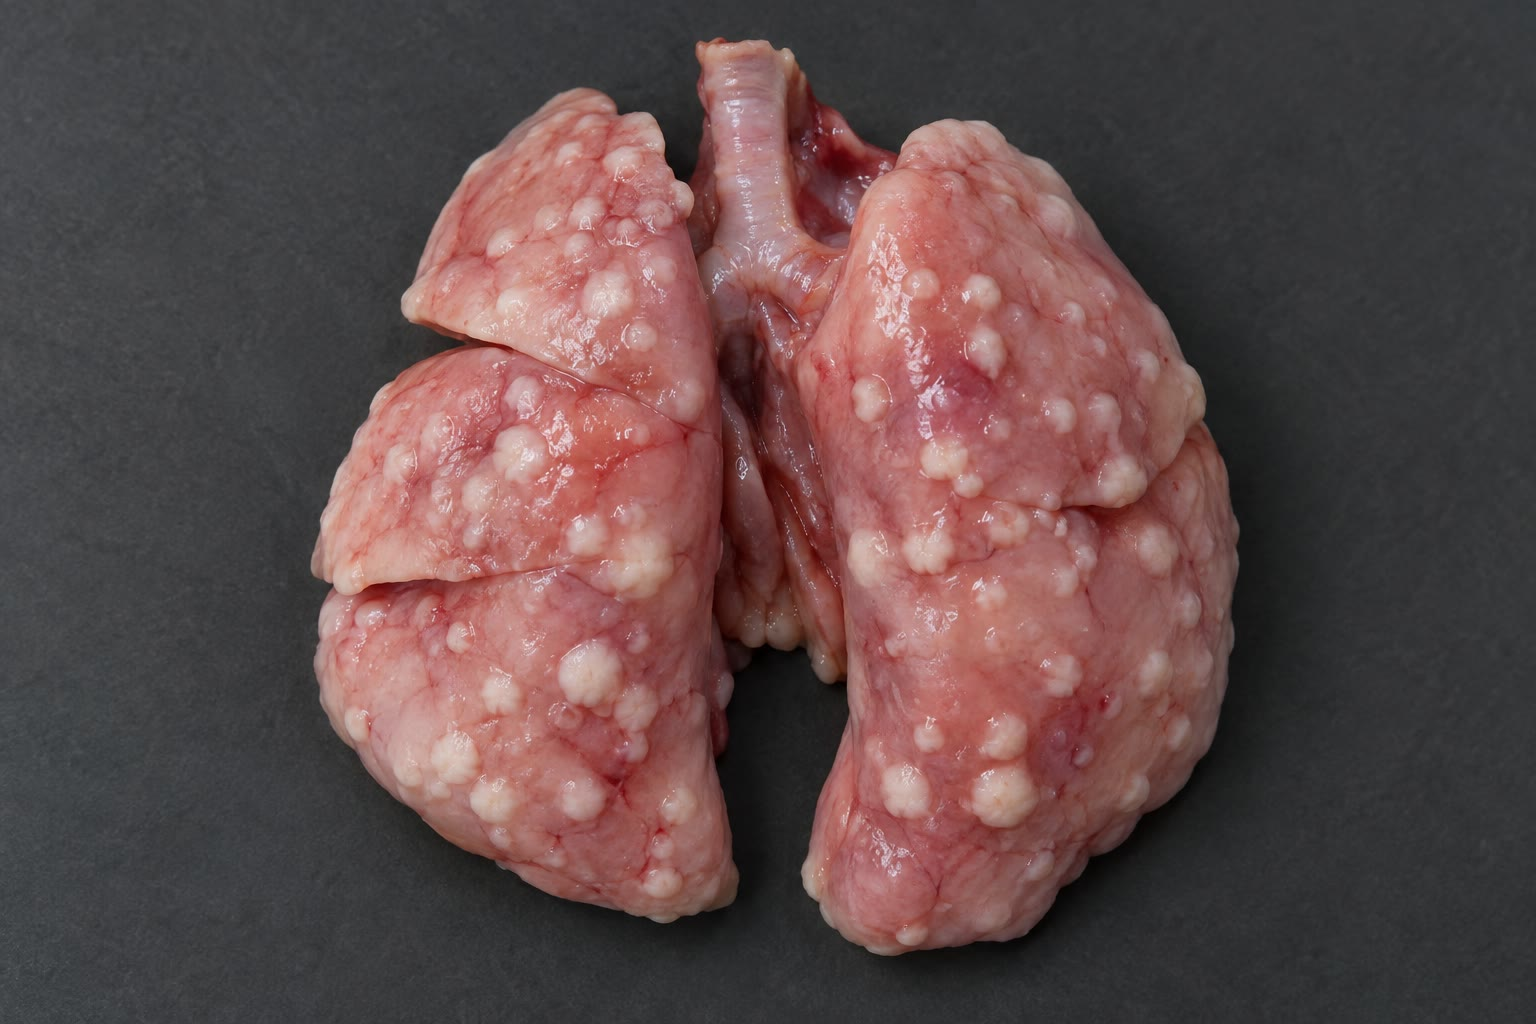
\includegraphics[width=0.54\linewidth]{images/book5/ai/b5-11-metastasis-lung.jpg}

{\small Izquierda: un esferoide tumoral (verde) que recluta vasos nuevos
(rojo) de una red vecina --- la angiogénesis en cultivo. Derecha: un
pulmón de ratón tachonado de \omterm{def:b3:cancer-biology:hallmarks}{metástasis}, cada colonia fundada por una
célula que sobrevivió al viaje por la sangre.}
\end{omfigure}

\begin{definition}[Invasión y metástasis]\label{def:b3:cancer-biology:metastasis}
\index{invasión}\index{transición epitelio--mesénquima}\index{semilla y suelo}
Para dar \omterm{def:b3:cancer-biology:hallmarks}{metástasis}, una célula de carcinoma ha de salir del epitelio ---
perder sus uniones celulares y su polaridad y adquirir motilidad, una
\emph{transición epitelio--mesénquima} impulsada por factores de
transcripción que normalmente se usan en el desarrollo embrionario ---,
degradar la membrana basal y la matriz con proteasas secretadas, cruzar
la pared de un vaso sanguíneo o linfático, sobrevivir en la circulación
(lo logran menos de una de cada diez mil, matadas por la cizalla, por la
falta de anclaje y por los linfocitos citolíticos naturales), alojarse en
un lecho capilar de otro órgano, salir de él y crecer allí. Dónde crece
no es aleatorio: el \omterm{def:b3:cancer-biology:hallmarks}{cáncer} de mama va al hueso, al pulmón, al hígado y al
cerebro; el de colon al hígado; el de próstata al hueso --- la
\emph{semilla y el suelo} de Paget, de 1889, explicados en parte por el
flujo sanguíneo y en parte por el encaje entre la célula y las señales
del tejido. Una célula diseminada puede quedar latente durante años antes
de crecer, que es por lo que los \omterm{def:b3:cancer-biology:hallmarks}{cánceres} reaparecen una década después
de una curación aparente. La \omterm{def:b3:cancer-biology:hallmarks}{metástasis} causa nueve de cada diez muertes
por \omterm{def:b3:cancer-biology:hallmarks}{tumores} sólidos, y es el paso peor comprendido.
\end{definition}

\begin{proposition}[Escapar del sistema inmunitario]\label{prop:b3:cancer-biology:immune}
\index{evasión inmunitaria}\index{inhibidor de puntos de control}\index{neoantígeno}
Las mutaciones de un \omterm{def:b3:cancer-biology:hallmarks}{tumor} crean \emph{neoantígenos}, péptidos que
ninguna célula normal presenta, y los linfocitos~T citotóxicos reconocen
y matan a las células tumorales --- la razón de que los pacientes
inmunodeprimidos tengan más \omterm{def:b3:cancer-biology:hallmarks}{cánceres} y de que los \omterm{def:b3:cancer-biology:hallmarks}{tumores} con muchas
mutaciones (melanoma, pulmón, colon deficiente en \omterm{prop:b3:dna-repair:fidelity}{reparación de errores
de apareamiento}) respondan mejor a la inmunoterapia. Un \omterm{def:b3:cancer-biology:hallmarks}{tumor} clínicamente
evidente es uno que ha escapado: perdiendo las moléculas del MHC que
presentan péptidos, secretando factores supresores, reclutando linfocitos
T reguladores y, sobre todo, expresando PD-L1, que engancha el receptor
inhibidor PD-1 de los linfocitos~T y los apaga, el mismo freno que
normalmente termina una respuesta inmunitaria
(\cref{ch:b3:adaptive-immunity}). Los anticuerpos que bloquean PD-1 o
PD-L1, o el freno anterior CTLA-4, sueltan a los linfocitos~T; en una
parte de los pacientes --- de una quinta parte a la mitad, según el \omterm{def:b3:cancer-biology:hallmarks}{tumor}
--- producen remisiones duraderas de \omterm{def:b3:cancer-biology:hallmarks}{cánceres} que eran intratables, y sus
efectos secundarios son autoinmunidad, la otra función del freno.
\end{proposition}

\section{Causas y tratamientos}

\begin{proposition}[Causas]\label{prop:b3:cancer-biology:causes}
\index{carcinógeno}\index{virus oncogénico}
El \omterm{def:b3:cancer-biology:hallmarks}{cáncer} lo causa todo lo que eleve la velocidad de los sucesos del
teorema o el número de células en riesgo. Los \emph{carcinógenos
químicos}, mutágenos casi todos ellos tras su activación por el hígado:
los setenta carcinógenos del humo del tabaco, que causan un tercio de las
muertes por \omterm{def:b3:cancer-biology:hallmarks}{cáncer} y elevan el riesgo de \omterm{def:b3:cancer-biology:hallmarks}{cáncer} de pulmón de quince a
veinticinco veces; la aflatoxina del grano enmohecido; el amianto, que no
es mutágeno sino un irritante crónico. La \emph{radiación}: la luz
ultravioleta para la piel (los dímeros del \cref{ch:b3:dna-repair}) y la
radiación ionizante para la leucemia, el tiroides y la mama. Las
\emph{infecciones}, una sexta parte de los \omterm{def:b3:cancer-biology:hallmarks}{cánceres} del mundo: los
papilomavirus, cuyas proteínas E6 y E7 destruyen \omterm{def:b3:cancer-biology:genes}{p53} e inactivan Rb y
causan casi todos los \omterm{def:b3:cancer-biology:hallmarks}{cánceres} de cuello uterino (una vacuna los previene
hoy); los virus de las hepatitis B y C en el \omterm{def:b3:cancer-biology:hallmarks}{cáncer} de hígado; el virus
de Epstein--Barr en los linfomas; \emph{Helicobacter pylori} en el \omterm{def:b3:cancer-biology:hallmarks}{cáncer}
de estómago, a través de décadas de inflamación. Las \emph{mutaciones
heredadas} de un supresor de \omterm{def:b3:cancer-biology:hallmarks}{tumores}, el primer golpe ya al nacer, en
cerca del \qty{5}{\%} de los \omterm{def:b3:cancer-biology:hallmarks}{cánceres}. Y el azar: la mayoría de las
mutaciones de un \omterm{def:b3:cancer-biology:hallmarks}{tumor} nacieron de los errores ordinarios de la
replicación, de modo que los tejidos que más se dividen --- colon, piel,
sangre --- son los que más \omterm{def:b3:cancer-biology:hallmarks}{cánceres} tienen, y el riesgo sube con la edad
haga uno lo que haga.
\end{proposition}

\begin{theorem}[Por qué un fármaco fracasa y dos pueden no hacerlo]\label{thm:b3:cancer-biology:goldie-coldman}
\index{modelo de Goldie--Coldman}\index{resistencia a fármacos}\index{terapia combinada}
Supóngase que un \omterm{def:b3:cancer-biology:hallmarks}{tumor} de $N$ células se ha producido por divisiones
sucesivas a partir de una sola célula, y que una mutación que confiere
resistencia a un fármaco dado surge a velocidad $\mu$ por división
celular. Entonces la probabilidad de que el \omterm{def:b3:cancer-biology:hallmarks}{tumor} \emph{no} contenga
ninguna célula resistente cuando empieza el tratamiento es
aproximadamente
\[
P_{0} \approx e^{-\mu N},
\]
de modo que para $\mu N \gg 1$ la resistencia preexiste con práctica
certeza. Para dos fármacos con mecanismos de resistencia independientes,
una célula resistente a ambos surge a velocidad aproximada
$\mu_{1}\mu_{2}$ por división, y $P_{0}
\approx e^{-\mu_{1}\mu_{2}N}$: con $N = 10^{9}$ y $\mu = 10^{-7}$, un
fármaco se enfrenta en promedio a $\mu N = 100$ clones resistentes, y dos
fármacos a una probabilidad de $10^{-5}$ de que exista siquiera una
célula doblemente resistente.
\end{theorem}
\begin{proof}[Demostración parcial]
Crecer de $1$ a $N$ células cuesta unas $N$ divisiones en total (un árbol
con $N$ hojas tiene $N - 1$ nodos internos). Si en cada división se
produce una célula resistente con probabilidad $\mu$ y, en primera
aproximación, sus descendientes ni mueren ni superan al resto, el número
de sucesos de resistencia sigue una Poisson de media $\mu N$, y la
probabilidad de que no haya ninguno es $e^{-\mu N}$. Los mecanismos
independientes multiplican las probabilidades por división. La
aproximación pasa por alto que los mutantes tempranos dejan clones
resistentes mayores --- la distribución completa es la de Luria y
Delbrück, tratada en el volumen de segundo año ---, pero la probabilidad
de que \emph{no} haya mutante, que es lo que decide si el \omterm{def:b3:cancer-biology:hallmarks}{tumor} puede
curarse, es exactamente el término de Poisson.
\end{proof}

\begin{example}[Las terapias y su lógica]\label{ex:b3:cancer-biology:therapy}
La cirugía y la radioterapia quitan o matan un \omterm{def:b3:cancer-biology:hallmarks}{tumor} localizado; la
radiación mata por \omterm{def:b3:dna-repair:lesions}{roturas de doble hebra}, y su fraccionamiento en dosis
diarias deja que el tejido normal repare entre ellas
(\cref{ch:b3:dna-repair}). La quimioterapia citotóxica --- agentes
alquilantes, antimetabolitos, venenos de los \omterm{def:b3:cytoskeleton-motility:filaments}{microtúbulos}, inhibidores de
topoisomerasas --- mata células en división de cualquier clase, las
tumorales algo más, y sigue una ley de \emph{muerte logarítmica}: cada
tanda mata una fracción constante, digamos el \qty{99}{\%}, de modo que
seis tandas reducen $10^{12}$ células a una, y hacen falta las mismas
seis tandas sea el \omterm{def:b3:cancer-biology:hallmarks}{tumor} grande o pequeño; el pelo, el intestino y la
médula del paciente, que también se dividen, fijan la dosis. La terapia
dirigida ataca una lesión de la que el \omterm{def:b3:cancer-biology:hallmarks}{tumor} depende: el imatinib bloquea
la quinasa BCR--ABL y convirtió la leucemia mieloide crónica de
enfermedad mortal en enfermedad crónica; el trastuzumab une HER2; los
inhibidores de PARP, los de Cdk4/6 y el venetoclax de capítulos
anteriores explotan cada uno un defecto. La inmunoterapia suelta a los
linfocitos~T. Y el teorema dice cómo deberían usarse: en combinación,
pronto, cuando $N$ es menor --- que es lo que hace la quimioterapia
adyuvante tras la cirugía --- y con fármacos cuyos mecanismos de
resistencia no se solapen. El \omterm{def:b3:cancer-biology:hallmarks}{tumor} es una población en evolución, y el
tratamiento es selección.
\end{example}

\begin{omfigure}
\begin{tikzpicture}
\begin{axis}[
  width=0.7\linewidth, height=5.6cm,
  axis x line=bottom, axis y line=left,
  xmin=0, xmax=8, ymin=1, ymax=1e13, ymode=log,
  xlabel={tandas de quimioterapia}, ylabel={células tumorales},
  xlabel style={font=\small, at={(axis description cs:0.5,-0.12)}, anchor=north},
  ylabel style={font=\small},
  tick label style={font=\small}, xtick={0,2,4,6,8},
  clip=false,
]
\addplot[very thick, omDef, mark=*, mark size=1.2pt] coordinates {(0,1e12) (1,1e10) (2,1e8) (3,1e6) (4,1e4) (5,1e2) (6,1)};
\addplot[very thick, omThm, mark=*, mark size=1.2pt] coordinates {(0,1e12) (1,1.01e10) (2,1.02e8) (3,1.04e6) (4,1.1e4) (5,200) (6,300) (7,600) (8,1200)};
\addplot[dashed, gray, domain=0:8, samples=2] {1e9};
\node[font=\scriptsize, gray, anchor=south west] at (axis cs:0.2,1.3e9) {detectable, $10^{9}$};
\node[font=\scriptsize, omDef, anchor=south west] at (axis cs:0.3,1e4) {\qty{99}{\%} de muerte por tanda};
\node[font=\scriptsize, omThm, anchor=south west] at (axis cs:5.2,3e3) {una célula resistente al principio: recaída};
\end{axis}
\end{tikzpicture}

{\small La ley de la muerte logarítmica. Cada tanda mata la misma
fracción de células, de modo que el \omterm{def:b3:cancer-biology:hallmarks}{tumor} se encoge un número fijo de
décadas por tanda y es indetectable mucho antes de haber desaparecido
(azul); una sola célula resistente preexistente sobrevive a todas las
tandas y vuelve a crecer (rojo).}
\end{omfigure}

\begin{remark}[Qué ha cambiado]\label{rem:b3:cancer-biology:changed}
La mitad de los pacientes a los que se diagnostica un \omterm{def:b3:cancer-biology:hallmarks}{cáncer} en un país
rico sobreviven hoy diez años, frente a una cuarta parte en 1970. La
ganancia vino de la prevención (el tabaco, las vacunas contra la
hepatitis y el papilomavirus, el cribado de pólipos y de lesiones del
cuello uterino), de la detección más temprana y de tratamientos que se
siguen de la biología de este capítulo --- la quimioterapia combinada que
cura la mayoría de las leucemias infantiles y de los \omterm{def:b3:cancer-biology:hallmarks}{cánceres} de
testículo, los fármacos dirigidos y las inmunoterapias. Lo que no ha
cambiado es la enfermedad metastásica, que la biología explica pero
todavía no cura; las próximas ganancias vendrán de tratar al \omterm{def:b3:cancer-biology:hallmarks}{tumor} como
lo que es, una población que evoluciona bajo la selección que impone el
tratamiento.
\end{remark}

\section{Ejercicios}

\begin{exercise}[$\star$]\label{exo:b3:cancer-biology:1}
Distíngase un \omterm{def:b3:cancer-biology:genes}{oncogén} de un \omterm{def:b3:cancer-biology:genes}{gen supresor de tumores} por su mecanismo, por
el número de alelos que han de cambiar, y con dos ejemplos de cada uno.
\end{exercise}

\begin{exercise}[$\star$]\label{exo:b3:cancer-biology:2}
Enumérense los \omterm{def:b3:cancer-biology:hallmarks}{rasgos distintivos del cáncer} y, para cada uno, nómbrese
un gen de este capítulo o de otro anterior cuya alteración lo aporta.
\end{exercise}

\begin{exercise}[$\star$]\label{exo:b3:cancer-biology:3}
¿Qué observó Knudson sobre el retinoblastoma hereditario y el esporádico,
y qué infirió?
\end{exercise}

\begin{exercise}[$\star$]\label{exo:b3:cancer-biology:4}
Explíquese la \omterm{met:b3:cancer-biology:ames}{prueba de Ames} y por qué se añade un extracto de hígado.
\end{exercise}

\begin{exercise}[$\star\star$]\label{exo:b3:cancer-biology:5}
La incidencia de un \omterm{def:b3:cancer-biology:hallmarks}{cáncer} es $2\times 10^{-5}$ al año a los $40$ años y
$2\times 10^{-3}$ a los $80$. Estímense el exponente de la ley de
potencias de la edad y el número de sucesos limitantes que sugiere.
\end{exercise}

\begin{exercise}[$\star\star$]\label{exo:b3:cancer-biology:6}
Con la \cref{prop:b3:cancer-biology:oxygen} y $D =
\qty{2e-9}{m^2/s}$ y $c_{0} = \qty{0.05}{mol/m^3}$, calcúlese $L$ para un
tejido que consume \qty{0.01}{mol/m^3/s} y para un \omterm{def:b3:cancer-biology:hallmarks}{tumor} que consume el
triple. ¿Por qué se vuelve necrótico antes un \omterm{def:b3:cancer-biology:hallmarks}{tumor} de crecimiento
rápido?
\end{exercise}

\begin{exercise}[$\star\star$]\label{exo:b3:cancer-biology:7}
Un \omterm{def:b3:cancer-biology:hallmarks}{tumor} de $10^{11}$ células se trata con un fármaco que mata el
\qty{99.9}{\%} por tanda. ¿Cuántas tandas hacen falta para reducirlo por
debajo de una célula? ¿Por qué el \omterm{def:b3:cancer-biology:hallmarks}{tumor} es indetectable tras dos tandas
aunque queden $10^{5}$ células, y qué implica eso para interrumpir el
tratamiento?
\end{exercise}

\begin{exercise}[$\star\star$]\label{exo:b3:cancer-biology:8}
Explíquese por qué rara vez se encuentran en el mismo \omterm{def:b3:cancer-biology:hallmarks}{tumor} de pulmón una
mutación de EGFR y otra de KRAS, y por qué un \omterm{def:b3:cancer-biology:hallmarks}{tumor} tratado con un
inhibidor de EGFR recae a menudo con una mutación de KRAS.
\end{exercise}

\begin{exercise}[$\star\star$]\label{exo:b3:cancer-biology:9}
Las proteínas E6 y E7 del papilomavirus inactivan \omterm{def:b3:cancer-biology:genes}{p53} y Rb. Explíquese
cómo esto impulsa el \omterm{def:b3:cancer-biology:hallmarks}{cáncer} de cuello uterino, por qué tarda décadas y
por qué una vacuna administrada antes de la actividad sexual lo previene.
\end{exercise}

\begin{exercise}[$\star\star\star$]\label{exo:b3:cancer-biology:10}
Extiéndase el argumento de Armitage--Doll para permitir que cada golpe
expanda su clon por un factor $g$ antes del siguiente: muéstrese que la
incidencia tiene la misma potencia de $t$ pero con el prefactor
multiplicado por $g^{k-1}$, y discútase por qué el $k$ ajustado a una
curva de edad es una cota superior del número de conductoras.
\end{exercise}

\begin{exercise}[$\star\star\star$]\label{exo:b3:cancer-biology:11}
Con el \cref{thm:b3:cancer-biology:goldie-coldman}, compárense (a) tratar
un \omterm{def:b3:cancer-biology:hallmarks}{tumor} de $10^{9}$ células con el fármaco A durante seis tandas y
después con el B durante otras seis, y (b) dar A y B juntos desde el
principio, cuando $\mu_{A} =
\mu_{B} = 10^{-7}$. Calcúlese $P_{0}$ para cada estrategia y explíquese
por qué la combinación temprana es la norma.
\end{exercise}

\begin{exercise}[$\star\star\star$]\label{exo:b3:cancer-biology:12}
La paradoja de Peto: un elefante tiene cien veces más células que una
persona y vive tanto como ella, y sin embargo no tiene más \omterm{def:b3:cancer-biology:hallmarks}{cáncer}. Con el
teorema de este capítulo, dígase cuál es la expectativa ingenua y
propónganse dos mecanismos con los que los animales grandes podrían haber
resuelto el problema (el elefante tiene veinte copias de \emph{TP53}).
\end{exercise}

\section{Problema: la aritmética de un tumor}

\begin{problem}[{Problema de fin de semana --- un tumor crecido a partir
de una célula y cronometrado hasta su detección, su curva de edad leída
para saber el número de golpes, su suministro de oxígeno y su núcleo
necrótico calculados, y su tratamiento planeado frente a la certeza de la
resistencia, hasta llegar a los años hasta la detección, al espesor de
tumor vivo alrededor de un vaso y a la probabilidad de que una
combinación cure}]
\label{pb:b3:cancer-biology:1}
Datos: una célula tumoral tiene un volumen de \qty{1000}{\micro m^3};
tiempo de duplicación, \qty{100}{d}; detección a \qty{1}{cm^3}; carga
letal, \qty{1}{kg}. Curva de edad: incidencia $1\times 10^{-5}$ al año a
los $30$ y $3\times
10^{-3}$ a los $80$. Oxígeno: $D = \qty{2e-9}{m^2/s}$, $c_{0} =
\qty{0.05}{mol/m^3}$,
$q = \qty{0.03}{mol/m^3/s}$ en el \omterm{def:b3:cancer-biology:hallmarks}{tumor}; en un \omterm{def:b3:cancer-biology:hallmarks}{tumor} vascularizado los
capilares están a \qty{150}{\micro m} unos de otros. Terapia: cada tanda
mata el \qty{99}{\%}; tasa de mutación de resistencia, $10^{-7}$ por
división y fármaco; una tanda cada tres semanas; el \omterm{def:b3:cancer-biology:hallmarks}{tumor} vuelve a crecer
entre tandas con el mismo tiempo de duplicación.

\medskip
\noindent\textbf{Parte I --- Crecimiento.}
\begin{enumerate}
  \item ¿Cuántas células hay en \qty{1}{cm^3}? ¿Cuántas duplicaciones a
        partir de una célula?
  \item ¿Cuántos años median entre la célula fundadora y la detección?
  \item ¿Cuántas duplicaciones, y cuántos años, van de la detección a la
        carga letal? Compárense los dos intervalos.
  \item Muchos \omterm{def:b3:cancer-biology:hallmarks}{tumores} se detectan a \qty{1}{cm^3} pero llevaban
        creciendo solo cinco años. ¿Qué debió de ocurrir con el tiempo de
        duplicación al principio, o con la ley de crecimiento?
  \item Solo una fracción $f$ de las células de un \omterm{def:b3:cancer-biology:hallmarks}{tumor} se está
        dividiendo en cada momento (la fracción de crecimiento), y otra
        fracción muere. Si las células ciclan en \qty{2}{d} pero el \omterm{def:b3:cancer-biology:hallmarks}{tumor}
        se duplica en $100$, ¿qué dice eso sobre el balance entre
        nacimientos y muertes?
  \item ¿Por qué la misma quimioterapia de muerte logarítmica respeta más
        a un \omterm{def:b3:cancer-biology:hallmarks}{tumor} de crecimiento lento que a uno rápido y, sin embargo,
        el rápido vuelve a crecer antes entre tandas?
\end{enumerate}

\medskip
\noindent\textbf{Parte II --- Golpes.}
\begin{enumerate}[resume]
  \item A partir de las dos incidencias, calcúlense el exponente $k - 1$
        de la curva de edad y el número implícito de sucesos $k$.
  \item Si cada suceso ocurre a $u = 10^{-6}$ por célula y año en
        $N = 10^{8}$ células susceptibles, ¿qué predice el teorema para
        el riesgo acumulado a los $70$ años con ese $k$? ¿Es verosímil?
        ¿Qué falta?
  \item Repítase con una expansión clonal por un factor $g = 100$ tras
        cada uno de los $k - 1$ primeros golpes, usando el
        \cref{exo:b3:cancer-biology:10}.
  \item Una portadora hereda un golpe. ¿Por qué factor sube su incidencia
        a los $40$ años, si las demás velocidades no cambian? (Compárese
        $(ut)^{k-1}$ con $(ut)^{k}$ en $t = 40$.)
  \item Fumar multiplica la $u$ de uno de los sucesos por $10$. ¿Por qué
        factor sube la incidencia si ese suceso es uno de los $k$? ¿Y si
        son dos de ellos?
  \item Explíquese por qué dejar de fumar a los cincuenta baja el riesgo
        de \omterm{def:b3:cancer-biology:hallmarks}{cáncer} de pulmón por debajo del de quien sigue fumando, pero
        nunca hasta el de quien nunca ha fumado.
\end{enumerate}

\medskip
\noindent\textbf{Parte III --- Suministro.}
\begin{enumerate}[resume]
  \item Calcúlese la profundidad de penetración del oxígeno $L$ en el
        \omterm{def:b3:cancer-biology:hallmarks}{tumor}.
  \item Un esferoide sin vasos: ¿cuál es el diámetro máximo con todas
        las células oxigenadas? ¿Cuál es el espesor del borde vivo de un
        esferoide de \qty{2}{mm}, y qué fracción de su volumen está
        viva?
  \item En un \omterm{def:b3:cancer-biology:hallmarks}{tumor} vascularizado con capilares separados
        \qty{150}{\micro m}, ¿están oxigenadas todas las células? ¿Qué
        células son hipóxicas, y por qué importa eso para la
        radioterapia (el oxígeno fija el daño de la radiación) y para la
        selección de células con \omterm{def:b3:cancer-biology:genes}{p53} mutante?
  \item Un fármaco reduce a la mitad la densidad capilar del \omterm{def:b3:cancer-biology:hallmarks}{tumor}.
        Recalcúlese la separación y dígase qué les ocurre a las células
        situadas a medio camino entre vasos.
  \item Las células hipóxicas pasan a la glicólisis y producen
        \qty{2}{ATP} por glucosa en lugar de $30$. ¿Por qué factor han de
        subir la captación de glucosa para mantener su suministro de ATP,
        y cómo se aprovecha esto para obtener imágenes de los \omterm{def:b3:cancer-biology:hallmarks}{tumores}?
  \item Explíquese por qué la terapia antiangiogénica por sí sola rara
        vez cura, pero puede ayudar a la quimioterapia a llegar al \omterm{def:b3:cancer-biology:hallmarks}{tumor}.
\end{enumerate}

\medskip
\noindent\textbf{Parte IV --- Tratamiento.}
\begin{enumerate}[resume]
  \item Un \omterm{def:b3:cancer-biology:hallmarks}{tumor} de \qty{1}{cm^3} se trata con un solo fármaco. ¿Cuántas
        tandas lo reducen por debajo de una célula, sin contar el
        recrecimiento ni la resistencia?
  \item Entre tandas (tres semanas) los supervivientes vuelven a crecer.
        ¿Por qué factor? Recalcúlense la muerte neta por ciclo y el
        número de ciclos necesarios.
  \item Calcúlense el número esperado de células resistentes al fármaco
        al empezar el tratamiento y la probabilidad de que no haya
        ninguna.
  \item Se dan juntos dos fármacos de mecanismos independientes.
        ¿Probabilidad de que no exista al principio ninguna célula
        doblemente resistente? ¿Y en un \omterm{def:b3:cancer-biology:hallmarks}{tumor} de $10^{12}$ células?
  \item La terapia adyuvante se da tras la cirugía, cuando quizá queden
        $10^{6}$ células sin detectar. Recalcúlense las probabilidades
        para uno y para dos fármacos, y enúnciese la lección.
  \item Una inmunoterapia induce linfocitos~T que matan a toda célula que
        presente un neoantígeno. ¿Por qué la resistencia a ella es un
        problema distinto de la resistencia a un inhibidor de quinasas, y
        en qué \omterm{def:b3:cancer-biology:hallmarks}{tumores} sugiere el teorema que debería funcionar mejor?
  \item Resúmase: los años que van de la célula fundadora a la detección
        (pregunta~2), el espesor de \omterm{def:b3:cancer-biology:hallmarks}{tumor} vivo alrededor de un vaso
        (pregunta~13) y la probabilidad de que la combinación de dos
        fármacos no encuentre ninguna célula resistente en un \omterm{def:b3:cancer-biology:hallmarks}{tumor} de
        \qty{1}{cm^3} (pregunta~22).
\end{enumerate}
\end{problem}
